% BEAMER ----
% This is just here so I know exactly what I'm looking at in Rstudio when messing with stuff.
\documentclass[12pt,ignorenonframetext,,aspectratio=149]{beamer}
\setbeamertemplate{caption}[numbered]
\setbeamertemplate{caption label separator}{: }
\setbeamercolor{caption name}{fg=normal text.fg}
\usepackage{lmodern}
\usepackage{amssymb,amsmath}
\usepackage{ifxetex,ifluatex}
\usepackage{fixltx2e} % provides \textsubscript
\ifnum 0\ifxetex 1\fi\ifluatex 1\fi=0 % if pdftex
  \usepackage[T1]{fontenc}
  \usepackage[utf8]{inputenc}
\else % if luatex or xelatex
  \ifxetex
    \usepackage{mathspec}
  \else
    \usepackage{fontspec}
  \fi
  \defaultfontfeatures{Ligatures=TeX,Scale=MatchLowercase}
  \newcommand{\euro}{€}
\fi
% use upquote if available, for straight quotes in verbatim environments
\IfFileExists{upquote.sty}{\usepackage{upquote}}{}
% use microtype if available
\IfFileExists{microtype.sty}{%
\usepackage{microtype}
\UseMicrotypeSet[protrusion]{basicmath} % disable protrusion for tt fonts
}{}

% Comment these out if you don't want a slide with just the
% part/section/subsection/subsubsection title:
\AtBeginPart{
  \let\insertpartnumber\relax
  \let\partname\relax
  \frame{\partpage}
}
\AtBeginSection{
  \let\insertsectionnumber\relax
  \let\sectionname\relax
  \frame{\sectionpage}
}
\AtBeginSubsection{
  \let\insertsubsectionnumber\relax
  \let\subsectionname\relax
  \frame{\subsectionpage}
}

\setlength{\emergencystretch}{3em}  % prevent overfull lines
\providecommand{\tightlist}{%
  \setlength{\itemsep}{0pt}\setlength{\parskip}{0pt}}
\setcounter{secnumdepth}{0}

\title{The Dangers of a Growing Anarchical Society}
\subtitle{DPR 190: War, Wealth, \& World Politics}
\author{Miles Williams}
\date{}


%% Here's everything I added.
%%--------------------------

\usepackage{graphicx}
\usepackage{rotating}
%\setbeamertemplate{caption}[numbered]
\usepackage{hyperref}
\usepackage{caption}
\usepackage[normalem]{ulem}
%\mode<presentation>
\usepackage{wasysym}
%\usepackage{amsmath}


% Get rid of navigation symbols.
%-------------------------------
\setbeamertemplate{navigation symbols}{}

% Optional institute tags and titlegraphic.
% Do feel free to change the titlegraphic if you don't want it as a Markdown field.
%----------------------------------------------------------------------------------
\institute{Data for Political Research}

% \titlegraphic{\includegraphics[width=0.3\paperwidth]{\string~/Dropbox/teaching/clemson-academic.png}} % <-- if you want to know what this looks like without it as a Markdown field.
% -----------------------------------------------------------------------------------------------------



% Some additional title page adjustments.
%----------------------------------------
\setbeamertemplate{title page}[empty]
%\date{}
\setbeamerfont{subtitle}{size=\small}

\setbeamercovered{transparent}

% Some optional colors. Change or add as you see fit.
%---------------------------------------------------
\definecolor{clemsonpurple}{HTML}{522D80}
 \definecolor{clemsonorange}{HTML}{F66733}
\definecolor{uiucblue}{HTML}{003C7D}
\definecolor{uiucorange}{HTML}{F47F24}





% Some optional color adjustments to Beamer. Change as you see fit.
%------------------------------------------------------------------
\setbeamercolor{frametitle}{fg=clemsonpurple,bg=white}
\setbeamercolor{title}{fg=clemsonpurple,,bg=white}
\setbeamercolor{local structure}{fg=clemsonpurple,}
\setbeamercolor{section in toc}{fg=clemsonpurple,bg=white}
% \setbeamercolor{subsection in toc}{fg=clemsonorange,bg=white}
\setbeamercolor{footline}{fg=clemsonpurple!50, bg=white}
\setbeamercolor{block title}{fg=clemsonorange,bg=white}


\let\Tiny=\tiny


% Sections and subsections should not get their own damn slide.
%--------------------------------------------------------------
\AtBeginPart{}
\AtBeginSection{}
\AtBeginSubsection{}
\AtBeginSubsubsection{}

% Suppress some of Markdown's weird default vertical spacing.
%------------------------------------------------------------
\setlength{\emergencystretch}{0em}  % prevent overfull lines
\setlength{\parskip}{0pt}


% Allow for those simple two-tone footlines I like.
% Edit the colors as you see fit.
%--------------------------------------------------
\defbeamertemplate*{footline}{my footline}{%
    \ifnum\insertpagenumber=1
    \hbox{%
        \begin{beamercolorbox}[wd=\paperwidth,ht=.8ex,dp=1ex,center]{}%
      % empty environment to raise height
        \end{beamercolorbox}%
    }%
    \vskip0pt%
    \else%
        \Tiny{%
            \hfill%
		\vspace*{1pt}%
            \insertframenumber/\inserttotalframenumber \hspace*{0.1cm}%
            \newline%
            \color{clemsonpurple}{\rule{\paperwidth}{0.4mm}}\newline%
            \color{clemsonorange}{\rule{\paperwidth}{.4mm}}%
        }%
    \fi%
}

% Various cosmetic things, though I must confess I forget what exactly these do and why I included them.
%-------------------------------------------------------------------------------------------------------
\setbeamercolor{structure}{fg=blue}
\setbeamercolor{local structure}{parent=structure}
\setbeamercolor{item projected}{parent=item,use=item,fg=clemsonpurple,bg=white}
\setbeamercolor{enumerate item}{parent=item}

% Adjust some item elements. More cosmetic things.
%-------------------------------------------------
\setbeamertemplate{itemize item}{\color{clemsonpurple}$\bullet$}
\setbeamertemplate{itemize subitem}{\color{clemsonpurple}\scriptsize{$\bullet$}}
\setbeamertemplate{itemize/enumerate body end}{\vspace{.6\baselineskip}} % So I'm less inclined to use \medskip and \bigskip in Markdown.

% Automatically center images
% ---------------------------
% Note: this is for ![](image.png) images
% Use "fig.align = "center" for R chunks

\usepackage{etoolbox}

\AtBeginDocument{%
  \letcs\oig{@orig\string\includegraphics}%
  \renewcommand<>\includegraphics[2][]{%
    \only#3{%
      {\centering\oig[{#1}]{#2}\par}%
    }%
  }%
}

% I think I've moved to xelatex now. Here's some stuff for that.
% --------------------------------------------------------------
% I could customize/generalize this more but the truth is it works for my circumstances.

\ifxetex
\setbeamerfont{title}{family=\fontspec{serif}}
\setbeamerfont{frametitle}{family=\fontspec{serif}}
\usepackage[font=small,skip=0pt]{caption}
 \else
 \fi

% Some random stuff now...
% ------------------------

\usepackage{tikz}

\newcommand{\shrug}[1][]{%
\begin{tikzpicture}[baseline,x=0.8\ht\strutbox,y=0.8\ht\strutbox,line width=0.125ex,#1]
\def\arm{(-2.5,0.95) to (-2,0.95) (-1.9,1) to (-1.5,0) (-1.35,0) to (-0.8,0)};
\draw \arm;
\draw[xscale=-1] \arm;
\def\headpart{(0.6,0) arc[start angle=-40, end angle=40,x radius=0.6,y radius=0.8]};
\draw \headpart;
\draw[xscale=-1] \headpart;
\def\eye{(-0.075,0.15) .. controls (0.02,0) .. (0.075,-0.15)};
\draw[shift={(-0.3,0.8)}] \eye;
\draw[shift={(0,0.85)}] \eye;
% draw mouth
\draw (-0.1,0.2) to [out=15,in=-100] (0.4,0.95);
\end{tikzpicture}}

% header includes go last.


% Okay, and begin the actual document...

\begin{document}
\frame{\titlepage}

\hypertarget{introduction}{%
\section{Introduction}\label{introduction}}

\begin{frame}{Introduction}
\protect\hypertarget{introduction-1}{}
We've been talking about the concept of sovereignty and how it gets
upheld in international politics. The idea of an ``anarchical society''
was brought up to explain the tension inherent to supporting a peaceful
state of affairs in international politics. In the anarchical society,
the society members are countries rather than individuals. As long as
these countries can agree to live and let live---that is, to respect the
sovereignty of each member---there will be peace.

\bigskip

The problem is that this society (a term that invokes ``order'' or
``rules'') lacks a central authority with a monopoly on the legitimate
use of violence to enforce the society's rules. Hence, the
\emph{anarchical} society. There are some measures that countries can
take to support order, like maintaining a balance of power or forming
alliances, but conflict is always lurking around the corner.
\end{frame}

\begin{frame}{Introduction}
\protect\hypertarget{introduction-2}{}
One point of tension that can threaten a peaceful state of affairs is
sudden shifts in the international system. In particular, if the number
of countries in the world changes, this can threaten a balance of power
or endanger a system of alliances if, say, one country turns into two or
more.

\bigskip

This leads to a clear conflict between competing principals. On the one
hand, the idea of self-determination sounds morally correct. If a group
of people want to form their own country and govern themselves however
they see fit, why shouldn't they have the right to do so? On the other
hand, the formation of a new country rarely is so simple. Many parties
can be affected both within and beyond the borders of the aspiring new
country. It is nearly impossible for a new country to emerge without it
leading to changes to international trade or geopolitical tensions.
\end{frame}

\hypertarget{a-hypothesis}{%
\section{A Hypothesis}\label{a-hypothesis}}

\begin{frame}{A Hypothesis}
\protect\hypertarget{a-hypothesis-1}{}
The tensions that inevitably surround the formation of new countries
gives us a basis for proposing and testing a \emph{hypothesis}. In the
field of International Relations, one of our jobs as researchers is to
study international politics through a \emph{scientific} lens. When we
look at the world and see a given event, we should seek not only to ask
``what is event {[}x{]} an example of?'' but also, ``if {[}x{]} is an
example of {[}y{]}, what else should we expect to happen?''

\bigskip

A hypothesis is a statement rooted in a theoretical argument about what
else we should expect to happen if {[}x{]} is an example of {[}y{]}. In
the case of our anarchical society, we know that one point of tension
that threatens the stability of the society is a change in the number of
its members. If this is true, what should we expect to see in the world
if the number of countries increases? We probably would see an increase
in conflict.
\end{frame}

\begin{frame}{A Hypothesis}
\protect\hypertarget{a-hypothesis-2}{}
So, based on this approach to understanding international politics, we
can propose a formal hypothesis:

\begin{quote}
\textbf{H:} \emph{An increase in the number of countries leads to an
increase in conflict.}
\end{quote}
\end{frame}

\hypertarget{testing-our-hypothesis}{%
\section{Testing our hypothesis}\label{testing-our-hypothesis}}

\begin{frame}{Testing our hypothesis}
\protect\hypertarget{testing-our-hypothesis-1}{}
The next thing we do as IR scholars is collect some data to test our
hypothesis. For many researchers, this data is quantitative in nature,
and we might use various data analysis tools to study it. This is
exactly what we can do to test our hypothesis that an increase in the
number of countries leads to an increase in conflict.

\bigskip

I collected and organized this data using some of my software. The next
few slides walk through what I found.
\end{frame}

\hypertarget{analysis}{%
\section{Analysis}\label{analysis}}

\begin{frame}{Analysis}
\protect\hypertarget{analysis-1}{}
First, I needed to calculate the number of countries in the world in a
given year. There's a lot of debate about who should count and different
approaches will give you slightly different totals. I decided to collect
some data from the Correlates of War conflict series. This is one of the
most authoritative datasets in IR for studying conflict among the
countries of the world. It covers the years 1816 to 2007.

\bigskip

The next slide shows what the number of countries in the world looks
like over this time-frame.
\end{frame}

\begin{frame}{Analysis}
\protect\hypertarget{analysis-2}{}
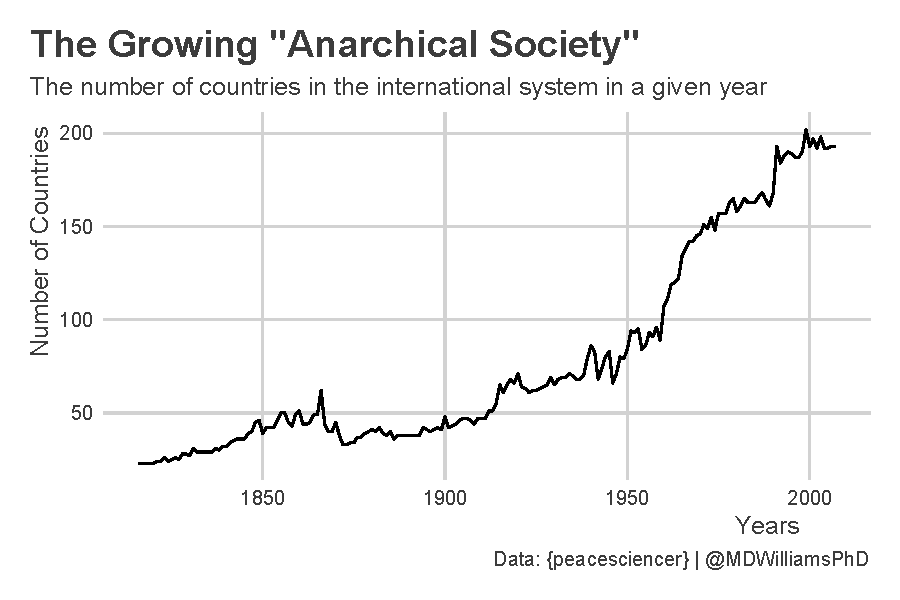
\includegraphics[width=0.95\linewidth]{figs/unnamed-chunk-1}
\end{frame}

\begin{frame}{Analysis}
\protect\hypertarget{analysis-3}{}
Now that we have a measure of the number of countries in the world, we
need a measure of the rate of conflict among these countries. To do
that, I used the same data source (Correlates of War). For each given
year, I counted the number of countries involved in some kind of war
(either a major international war or a intra-state war, also called a
civil war) that started in a given year. I then divided this total by
the total number of countries in the world at a given time. This gives
me a rate of conflict initiation in a given year per the number of
countries in the international system. The next slide shows how the
conflict rate varies over time.
\end{frame}

\begin{frame}{Analysis}
\protect\hypertarget{analysis-4}{}
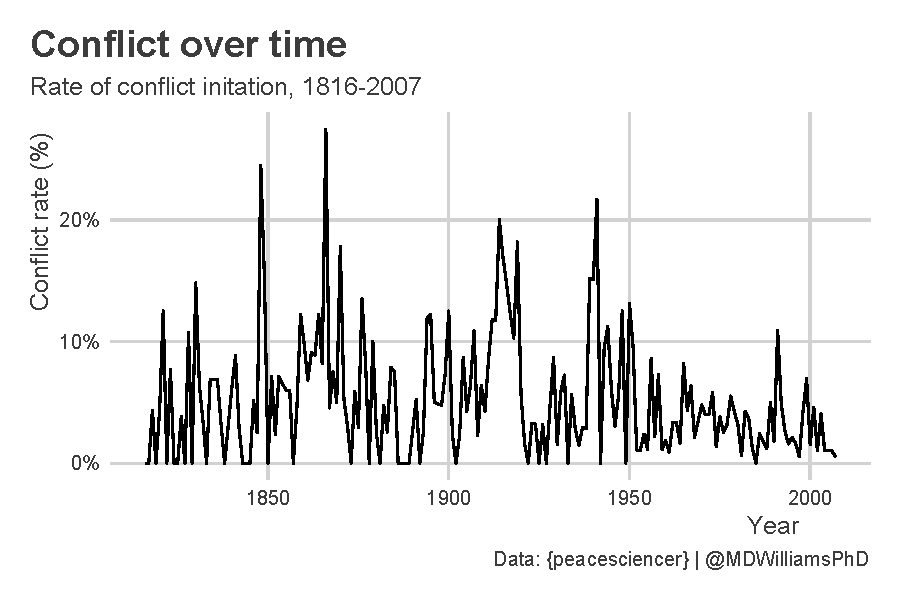
\includegraphics[width=0.95\linewidth]{figs/unnamed-chunk-2}
\end{frame}

\begin{frame}{Analysis}
\protect\hypertarget{analysis-5}{}
The next thing to do is examine the correlation between the number of
countries and conflict. I don't want to just look at the correlation
between \emph{total} countries and conflict, though. Our hypothesis is
founded on the idea that a \emph{change} in the number of countries is
what leads to more conflict. So, before we look at the correlation, we
need to transform the data to calculate the change in the number of
countries in the world in a given year.

\bigskip

After making this transformation, the next slide shows what the data
tell us.
\end{frame}

\begin{frame}{Analysis}
\protect\hypertarget{analysis-6}{}
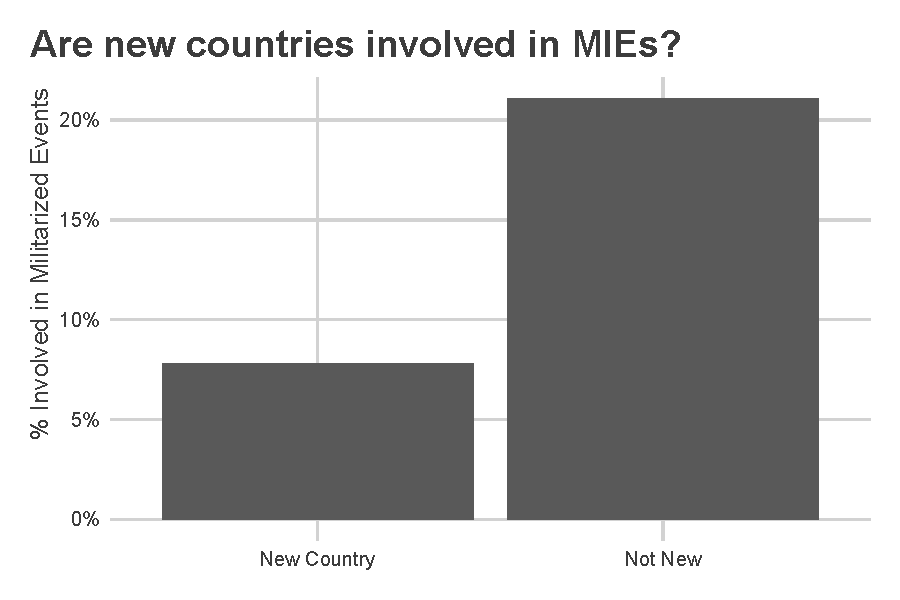
\includegraphics[width=0.95\linewidth]{figs/unnamed-chunk-3}
\end{frame}

\begin{frame}{Analysis}
\protect\hypertarget{analysis-7}{}
What does the data tell us? Does it support our hypothesis? The answer
is ``yes.'' An increase in the number of countries has a positive
correlation with the rate of conflict in the world.

\bigskip

Of course, there are always other factors to consider. Things that we
don't observe in the data (important events, trends in other variables,
etc.) could make it look like the correlation between the change in the
number of countries and conflict is positive when, in fact, the truth is
that one doesn't have anything to do with the other.

\bigskip

Even so, at least at first glance, the data support our hypothesis. By
extension, that means the data support the value of our broader
framework of characterizing the state of affairs among countries as an
anarchical society.
\end{frame}

\hypertarget{review}{%
\section{Review}\label{review}}

\begin{frame}{Review}
\protect\hypertarget{review-1}{}
In review:

\begin{itemize}
\tightlist
\item
  We talked about sovereignty and the tensions inherent to respecting
  sovereignty among members of an anarchical society.
\item
  We put on our IR scholar hats and approached this issue from a
  scientific perspective.
\item
  We reasoned that an increase in the number of countries in the world
  would lead to an increase in violence.
\item
  We tested this hypothesis using data and the data supported our
  hypothesis.
\end{itemize}

The real practice of research in IR is more complicated than this, but
this should give you a helpful model of what the process looks like.
\end{frame}


\section[]{}
\frame{\small \frametitle{Table of Contents}
\tableofcontents}
\end{document}
